\section{Solución desarrollo}
\subsection{Actividad 1}

\noindent\textbf{1. Encontrar la representación mediante el patrón de polos y ceros, así como el término constante del sistema cuya función de transferencia es:}
	\begin{equation}
		H(s)=\frac{6s^2+18s+12}{2s^3+10s^2+16s+12}
	\end{equation}
	\newline
	
	Término constante
	\begin{equation}
		H(s)=\frac{6s^2+18s+12}{2s^3+10s^2+16s+12}
	\end{equation}
	\begin{equation}
		\Rightarrow H(s)=\frac{6*\frac{6s^2}{6}+\frac{18s}{6}+\frac{12}{6}}{2*\frac{2s^3}{2}+\frac{10s^2}{2}+\frac{16s}{2}+\frac{12}{2}}
	\end{equation}
	\begin{equation}
		\Rightarrow H(s)=\frac{6*(s^2+3s+2)}{2*(s^3+5s^2+8s+6)}
	\end{equation}
	\begin{equation}
		\Rightarrow H(s)=3*\frac{s^2+3s+2}{s^3+5s^2+8s+6}
	\end{equation}	
	\begin{equation}
		\Rightarrow Termino Constante = 3
	\end{equation}
	
	Raíces
	\begin{equation}
		H(s)=\frac{s^2+3s+2}{s^3+5s^2+8s+6}
	\end{equation}	
	\begin{equation}
		\Rightarrow H(s)=\frac{(s+2)(s+1)}{(s+3)(s^2+2s+2)}
	\end{equation}		
	\begin{equation}
		\Rightarrow c_1=-2,c_2=-1,c_3=-3,c_4=1+\iu,c_5=1-\iu
	\end{equation}		
	
	\noindent Debido a que los polos son las raíces del denominador y los ceros las raíces del numerador llegamos a que
	\begin{equation}
		Ceros: c_1=-2,c_2=-1 
	\end{equation}		
	\begin{equation}
		Polos: c_3=-3,c_4=1+\iu,c_5=1-\iu
	\end{equation}
	\newline
	
\subsection{Actividad 2}

\subsection{Actividad 3}
\noindent\textbf{3. De la Figura 20 obtenga la ecuación diferencial que represente la dinámica del sistema.}	
\[
f(t)=x(t){\Longrightarrow}Entrada.
\]
\[
x=y(t){\Longrightarrow}Salida.
\]
\[
m:masa.
\]
\[
b:fricción.
\]
\[
f(t)-m{\"x}-b{\.x}=0
\]
\[
f(t)=m{\"x}+b{\.x}
\]
\[
\therefore x(t)=m{\"y}+b{\.y}
\]


\subsection{Actividad 4}
	
	\noindent\textbf{4.  Obtenga la función de transferencia del sistema y determine la expresión matemática de la respuesta impulso unitario (considere condiciones iniciales nulas):
	\begin{equation}
		S=\frac{1}{ms^2+bs}=\frac{1}{s(ms+b)=\frac{A}{s}+\frac{B}{ms+b}}
	\end{equation}
	\begin{equation}
		\Rightarrow 1=A(ms+b)+Bs
	\end{equation}
	Si s = 0
	\begin{equation}
		\Rightarrow 1=A(m*0+b)+B*0
	\end{equation}
	\begin{equation}
		\Rightarrow 1=A(b)
	\end{equation}
	\begin{equation}
		\Rightarrow A=\frac{1}{b}
	\end{equation}
	Si s=$\frac{-b}{m}$
	\begin{equation}
		\Rightarrow 1=A(m*\frac{-b}{m}+b)+B(\frac{-b}{m})
	\end{equation}
	\begin{equation}
		\Rightarrow 1=A(-b+b)+B(\frac{-b}{m})
	\end{equation}
	\begin{equation}
		\Rightarrow 1=A(0)+B(\frac{-b}{m})
	\end{equation}
	\begin{equation}
		\Rightarrow 1=B(\frac{-b}{m})
	\end{equation}
	\begin{equation}
		\Rightarrow B=\frac{m}{-b}
	\end{equation}
	Por lo tanto, tras sustituir A y B obtenemos
	\begin{equation}
		S=\frac{1}{s(b)}-\frac{-m}{b(ms+b)}=\frac{1}{b}\frac{1}{s}-\frac{m}{mb}\frac{1}{s+\frac{b}{m}}
	\end{equation}
	Si aplicamos función de Laplace inversa a este resultado obtenemos
	\begin{equation}
		y(t)=\frac{1}{b}u(t)-\frac{1}{b}e^{-\frac{b}{m}*t}
	\end{equation}
	\newline
	
\subsection{Actividad 5}

\subsection{Actividad 6}
\noindent\textbf{6. Considere un sistema cuya función de transferencia es representada como:
\[
F(s)=\frac{s+1}{s(s+2)}
\]
Utilice el método de fracciones parciales para encontrar la transformada inversa de Laplace y corrobore sus resultados con ayuda de un software especializado.}	
\[
\frac{s+1}{s(s+2)}=\frac{A}{s}+\frac{B}{s+2}{\Longrightarrow}(1)
\]
Multiplicamos la expresión (1) por s(s+2).
\[
(\frac{s+1}{s(s+2)})*s(s+2)=(\frac{A}{s}+\frac{B}{s+2})*s(s+2)
\]
\[
s+1=A*(s+2)+B*(s){\Longrightarrow}(2)
\]
Para poder encontar los valores de A y B primeramente vamos a sustituir de la expresión (2) los valores de s por 0, y vamos a resolver.
\[
\textbf{s=0:}
\]
\[
s+1=A*(s+2)+B*(s)
\]
\[
0+1=A*(0+2)+B*(0)
\]
\[
1=A*2
\]
\[
\frac{1}{2}=A
\]
\[
\therefore A=\frac{1}{2}
\]
Para poder encontrar el valor de B, vamos a sustituir el valor de s, igualmente de la expresión (2) por -1, y vamos a resolver.
\[
\textbf{s=-1:}
\]
\[
s+1=A*(s+2)+B*(s)
\]
\[
-1+1=A*(-1+2)+B*(-1)
\]
\[
0=A*(1)-B
\]
\[
0=A-B
\]
\[
A=B
\]
\[
\therefore B=\frac{1}{2}
\]
Sustituimos los valores de A y B en la expresión (1).
\[
\frac{s+1}{s(s+2)}=\frac{\frac{1}{2}}{s}+\frac{\frac{1}{2}}{s+2}
\]
\[
F(s)=\frac{1}{2}\frac{1}{s}+\frac{1}{2}\frac{1}{s+2}
\]
\[
\mathcal{L}^{-1}=\mathcal{L}^{-1}
\]
\[
\therefore{y(t)=\frac{1}{2}\mathscr{U}(t)+\frac{1}{2}e^{-2t}}
\]
Comprobación en MATLAB:
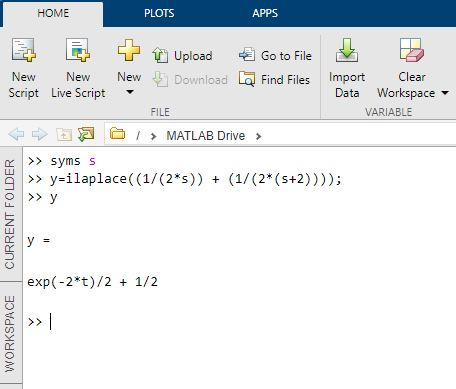
\includegraphics[scale=0.8, angle=0]{mAT.JPG}

\subsection{Actividad 7}
\subsection{Actividad 8}

\subsection{Actividad 9}
\noindent\textbf{9. De una forma alternativa, considerando el teorema del valor final y el teorema del valor inicial (sin la transformada inversa de Laplace) determine la respuesta al escalón. ¿Qué puede decir con respecto a lo realizado en la actividad 8?.}
\[
y(s)=\frac{3s+1}{s(5s+1)}
\]
\[
\lim_{s \to \infty}y(s)=\lim_{s \to \infty}\frac{3s+1}{s(5s+1)}
\]
\[
\lim_{s \to 0}y(s)=\lim_{s \to 0}\frac{3s+1}{s(5s+1)}
\]
Para poder utilizar el teorema del valor inicial y del valor final, debemos hacer que nuestra expresión tenga la siguiente estructura:
\[
H(s)=\frac{1}{s}\frac{bs+c}{(s+a)}
\]
Para ello vamos a dividir tanto el numerador como denominador entre 5, y vamos a reacomodar.
\[
=\frac{\frac{1}{5}}{\frac{1}{5}}\frac{3s+1}{s(5s+1)}
\]
\[
=\frac{\frac{3s+1}{5}}{s{\frac{5s+1}{5}}}
\]
\[
=\frac{1}{s}\frac{\frac{3}{5}s+\frac{1}{5}}{s+\frac{1}{5}}
\]
\[
a=\frac{1}{5};b=\frac{3}{5};c=\frac{1}{5}
\]
Una vez que tenemos nuestra  expresión con la estructura de H(s), vamos a ver que por definición tenemos lo siguiente:
\[
H(\infty)=b
\]
\[
H(0)=\frac{c}{a}
\]
Por lo tanto:
\[
\lim_{s \to \infty}y(s)=H(\infty)=b=\frac{3}{5}=0.6
\]
\[
\lim_{s \to 0}y(s)=H(0)=\frac{c}{a}=\frac{\frac{1}{5}}{\frac{1}{5}}=
\frac{5*1}{5*1}=1
\]
A través del teorema del valor inicial y el valor final, podemos llegar a los mismos valores (inicial y final), y esto se puede comprobar con la grafica obtenida en el inciso 8), ya que muestra los mismos valores.
